\documentclass{article}

\usepackage{listings,font spec,tikz}
\setmainfont[Ligatures=TeX]{Garamond}
\setsansfont[Scale=0.9]{Avenir Next}
\setmonofont[Scale=0.9]{Source Code Pro}

\lstset{language=python,basicstyle=\ttfamily,backgroundcolor=\color{black!10!white},frame=single,tabsize=2}

\begin{document}

\title{Perfidious ATM documentation}
\author{Liam Kelley and Shayan Amir-Kabirian}
\date{\today}
\maketitle

\section*{Summary}
To see normal features of the ATM program, use the PIN \texttt{1234}. To see easter eggs, try the PIN \texttt{8267}.

\section{Program Logic Structure}
The program, instead of running as a continuous \texttt{while} loop, runs as a series of functions. There are functions for displaying the menu and functions for each of the menu options, such as Deposit or Withdrawal. These functions, when finished, then call menu again. The overall logic is as follows:

\begin{figure}[h!]
\centering
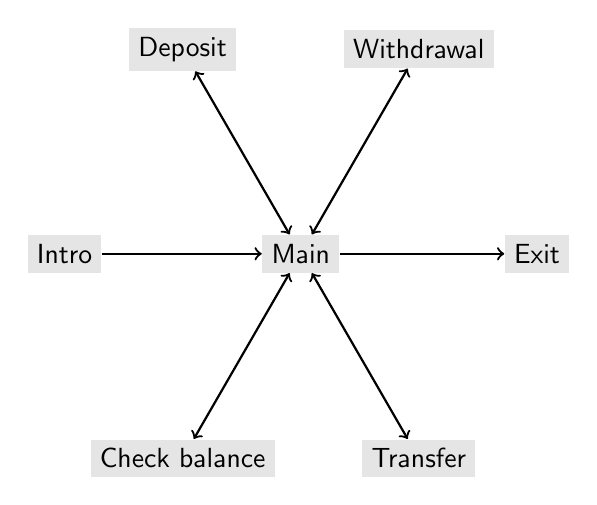
\begin{tikzpicture}[font=\sffamily]
	% NODES
	\tikzset{every node/.style={fill=black!10!white}}
	\node (i) at (-3,0) {Intro};
	\node (m) at (0,0) {Main};
	\node (w) at (60:3) {Withdrawal};
	\node (d) at (120:3) {Deposit};
	\node (c) at (-120:3) {Check balance};
	\node (t) at (-60:3) {Transfer};
	\node (e) at (3,0) {Exit};
	
	% ARROWS
	\draw[->,thick] (i) -- (m);
	\draw[<->,thick] (m) -- (d);
	\draw[<->,thick] (m) -- (w);
	\draw[<->,thick] (m) -- (c);
	\draw[<->,thick] (m) -- (t);
	\draw[->,thick] (m) -- (e);
\end{tikzpicture}

\caption{Function logic}
\end{figure}

The use of functions leads to potential issues with global variables, especially the balances of the two accounts. To overcome this issue, we pass the values of checking and savings along as inputs to each menu option. Therefore, calling the menu requires:
\begin{lstlisting}
main(checking_account,savings_account)
\end{lstlisting}
Calling the deposit function, as another example, also requires the two accounts as inputs.
\begin{lstlisting}
deposit(checking_account,savings_account)
\end{lstlisting}
By passing the account information along to each menu, we avoid having to make \texttt{checking\_account} and \texttt{savings\_account} global variables.

\section{Additional Features and Easter Eggs}
The ATM is itself fully functional, but seems a touch off . This is intentional, of course. The ATM is vaguely Germanic, with umlauts over many of the u's, and the use of Euro instead of USD. Furthermore, the company is meant to sound sketchy. Perfidious means ``deceitful and untrustworthy,'' and the company name itself changes over the course of the program. Each time the program says the name, the classification at the end of the company (i.e. Inc., LLC, etc.) is randomly generated using the following code:
\begin{lstlisting}[numbers=left]
def bank_name():
  n = random.randint(0,18)
  title = "GmbH","AG","AG & Co. KG" # rest left off for brevity
  return "Perfidious Banking Group, " + title[n]
\end{lstlisting}
The name is therefore thrown in by calling \texttt{bank\_name()} in a \texttt{print()} statement.

Certain features of the ATM were made more advanced. PINs, of which there are four, are read from a file instead of hardcoded into the program. Similarly, the account information is also stored in a separate file, as is the build number. Therefore, code was implemented for reading the file and rewriting the information within, for the account information and the build number. The build number was read and iterated by one. The function that reads and outputs the build number is below as an example of text file I/O.
\begin{lstlisting}[numbers=left]
def build():
  build_file = open('build.txt','r')
  build_num = build_file.readline()
  build_num = int(build_num.rstrip("\n"))
  new_build = build_num + 1
  build_file = open('build.txt', 'w')
  build_file.write(str(new_build)+"\n")
  return new_build
\end{lstlisting}
The documentation of each line in the function is included as comments in the program itself. As a result, the PINs, build number, and account information are all stored in \texttt{.txt} documents that the functions reads and rewrites as necessary. For account information, the account balances are read when the program is initialized and rewritten when the program exits.

The basic functionality of program is available for the default PIN, which is \texttt{1234}. However, there are also three administrator PINs, which are \texttt{1248}, \texttt{3333}, and \texttt{8267}. These correspond to Liam, Shayan, and our friend RC. Inputting any of these PINs allows for access to an admin menu with some farcical illegal options, such as money laundering. Additionally, because our friend RC has a cherished lobster stuffed animal, there is a verification that the user is a person and not a lobster. If the user is a lobster, the program exits immediately.

The admin menu has a similar overall structure to the main menu. The options for the admin menu, which are:
\begin{enumerate}
	\item Quick Money Laundering
	\item Transfer to Cayman Account
	\item Fast Embezzle €1000
	\item Delete All Evidence
	\item Return to Main Menu
\end{enumerate}
These menu options are called in the same general way that main menu functions are called. The admin menu itself is only an option in the main menu when the global toggle \texttt{admin} is set to \texttt{True}, which occurs when an admin PIN is entered. The logic of each admin menu option is still very basic and related to normal menu options. Money laundering and transfer to Cayman account utilize the same general logic as the withdrawal function, while fast embezzle uses the same logic as deposit. Delete all evidence utilizes the same general logic as the exit functionality, and rewrites the account file to be blank (it also adds a little showmanship).

There are also two defined functions that are never called, which is a good thing because they are intentional infinite loops. The function \texttt{meow()} prints ``meow'' repeatedly.
\begin{lstlisting}[numbers=left]
def meow():
  meow = "meow"
  while meow == "meow":
    print(meow)
\end{lstlisting}
Meanwhile, the function \texttt{conjure\_puppies()} prints ``Puppies!'' until the end of time, or at least until it is forcibly stopped.
\begin{lstlisting}[numbers=left]
def conjure_puppies():
  puppy_cuteness = True
  while puppy_cuteness:
    print("Puppies!")
\end{lstlisting}

\end{document}